\documentclass[10pt]{article}
\usepackage[margin=1in]{geometry}
\usepackage{amsmath,amssymb,amsthm}
\usepackage{graphicx}
\usepackage{subcaption}
\usepackage{booktabs}
\usepackage{hyperref}
\usepackage{xcolor}
\usepackage{caption}
\hypersetup{colorlinks=true,linkcolor=blue!60!black,citecolor=blue!60!black}

\graphicspath{{../results/}}

\title{ECE 66200 Project 2:\\
Orthogonal Low-Rank Transformation (OLT)}
\author{Weiheng Tang}
\date{\today}

\newcommand{\T}{\mathbf{T}}
\newcommand{\Y}{\mathbf{Y}}
\newcommand{\F}{\mathbf{F}}
\newcommand{\X}{\mathbf{X}}
\DeclareMathOperator*{\argmin}{arg\,min}
\newcommand{\nuc}[1]{\left\|#1\right\|_{\ast}}
\newcommand{\spn}[1]{\left\|#1\right\|_{2}}

\begin{document}
\maketitle

\section{Problem formulation and OLT objective}

Given $C$ classes of samples $\Y = [\Y_1,\dots,\Y_C]$ where $\Y_c \in
\mathbb{R}^{d\times n_c}$ stacks the $n_c$ samples of class $c$ as
columns, the Orthogonal Low-rank Transformation (OLT) seeks a linear
map $\T \in \mathbb{R}^{d'\times d}$ that simultaneously
\emph{compresses each class to a low-rank subspace} and \emph{makes
those subspaces mutually orthogonal}. Both goals are encoded through a
single nuclear-norm based objective:
\begin{equation}
\min_{\T}\;\;
\sum_{c=1}^{C}\nuc{\T \Y_c}\;-\;\nuc{\T \Y}
\quad\text{s.t.}\quad \spn{\T}=1.
\label{eq:olt}
\end{equation}
The constraint $\spn{\T}=1$ rules out the trivial scaling $\T\to 0$.

\paragraph{Why this objective.} The nuclear norm $\nuc{A}=\sum_i
\sigma_i(A)$ is the tightest convex surrogate of $\mathrm{rank}(A)$, so
$\sum_c\nuc{\T\Y_c}$ acts as a class-wise rank surrogate
(\emph{intra-class compression}). Furthermore, for any block matrix
$[A,B]$ one has the standard inequality
\begin{equation}
\nuc{[A,B]}\;\le\;\nuc{A}+\nuc{B},\qquad
\text{with equality iff } \mathrm{col}(A)\perp\mathrm{col}(B),
\label{eq:perp}
\end{equation}
so the gap $\sum_c\nuc{\T\Y_c}-\nuc{\T\Y}\ge 0$, and the gap vanishes
\emph{exactly} when the transformed class subspaces are pairwise
orthogonal. Minimising the gap therefore drives both rank reduction and
inter-class orthogonality with one term.

\section{Optimization via the Concave--Convex Procedure (CCCP)}
\label{sec:cccp}

The objective in \eqref{eq:olt} is a difference of two convex functions
\[
f(\T)=u(\T)-v(\T),\qquad
u(\T)=\sum_c\nuc{\T\Y_c},\qquad
v(\T)=\nuc{\T\Y}.
\]
CCCP linearises the concave term $-v(\T)$ around the current iterate
$\T^{(t)}$. With the chain rule and the subgradient rule for nuclear
norms,
\[
\frac{\partial}{\partial \T}\nuc{\T\Y}\;=\;G\,\Y^{\top},
\qquad
\Y^{\top}\T^{\top}=U\Sigma V^{\top}\;\Rightarrow\;G=UV^{\top},
\]
the linearised subproblem becomes
\begin{equation}
\T^{(t+1)}=\argmin_{\T}\;\sum_c\nuc{\T\Y_c}\;-\;\mathrm{tr}\!\left(G\,\Y^{\top}\T^{\top}\right),
\quad\spn{\T}=1,
\label{eq:cccp_inner}
\end{equation}
solved by a few proximal subgradient steps followed by a projection
$\T\leftarrow\T/\sigma_{\max}(\T)$ to enforce the constraint. We
implement this in \texttt{olt/solver.py}; gradients are scaled by
$1/N$ so that the step size is dataset-size invariant.

\section{Part 1: OLT with the nuclear norm}

\subsection{Task 1 -- Toy datasets}

We follow the starter notebook and generate synthetic data on
non-orthogonal 1D subspaces in $\mathbb{R}^{2}$ (two classes) and
$\mathbb{R}^{3}$ (three classes). After running CCCP we measure (i) the
absolute cosine matrix between per-class top principal directions and
(ii) per-class singular values of the transformed features.

\begin{figure}[h]
\centering
\begin{subfigure}[t]{0.34\linewidth}
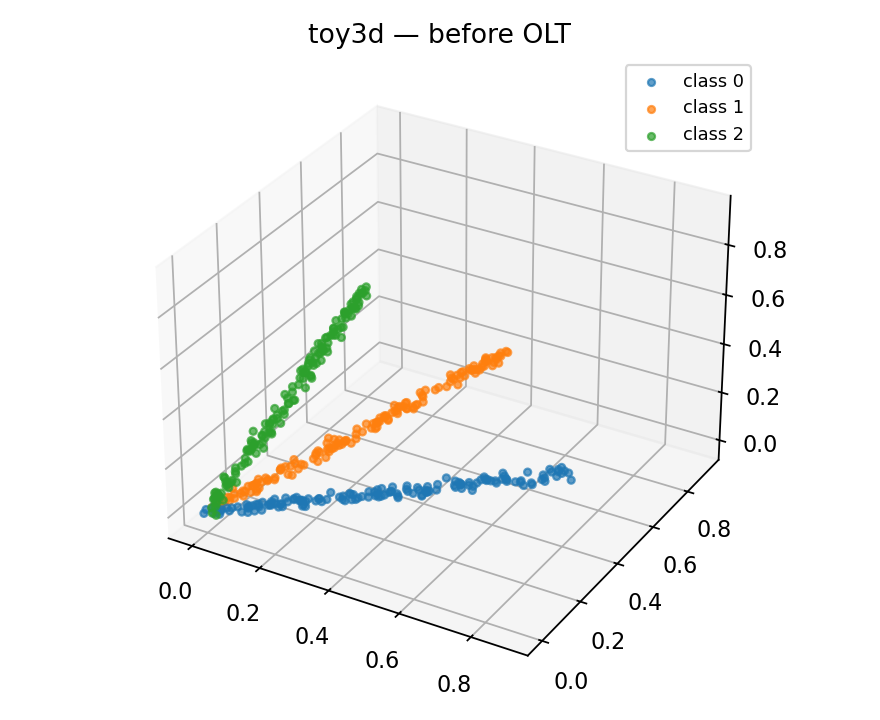
\includegraphics[width=\linewidth]{part1_toy/toy3d_before.png}\caption{Before}
\end{subfigure}
\begin{subfigure}[t]{0.34\linewidth}
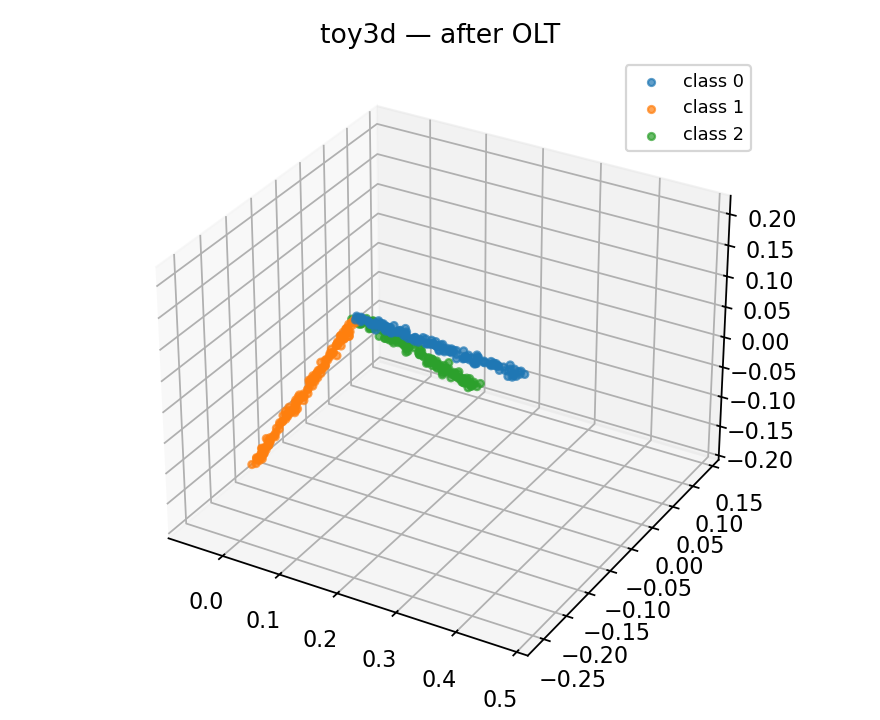
\includegraphics[width=\linewidth]{part1_toy/toy3d_after.png}\caption{After OLT}
\end{subfigure}
\begin{subfigure}[t]{0.27\linewidth}
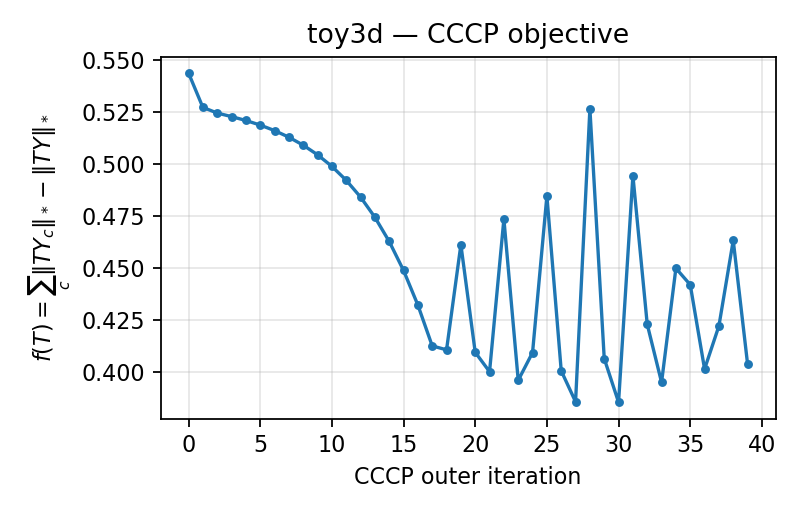
\includegraphics[width=\linewidth]{part1_toy/toy3d_obj.png}\caption{CCCP objective}
\end{subfigure}\\[0.4em]
\begin{subfigure}[t]{0.30\linewidth}
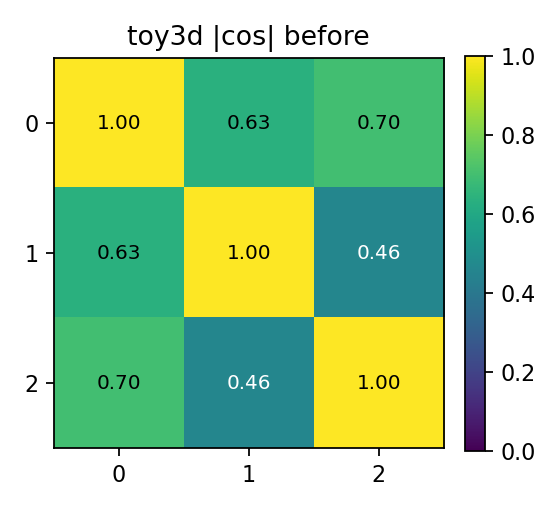
\includegraphics[width=\linewidth]{part1_toy/toy3d_cos_before.png}\caption{$|\cos|$ before}
\end{subfigure}
\begin{subfigure}[t]{0.30\linewidth}
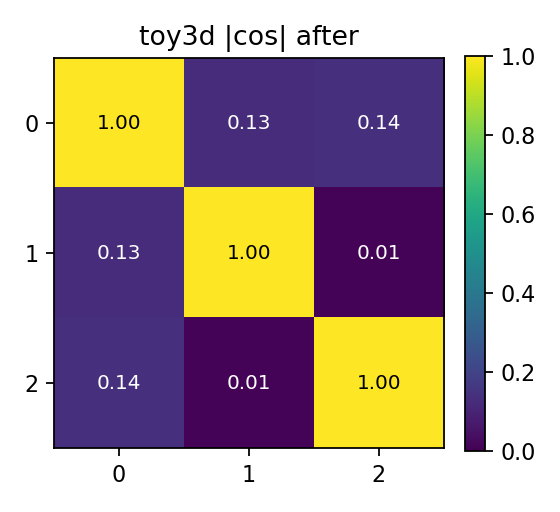
\includegraphics[width=\linewidth]{part1_toy/toy3d_cos_after.png}\caption{$|\cos|$ after}
\end{subfigure}
\begin{subfigure}[t]{0.34\linewidth}
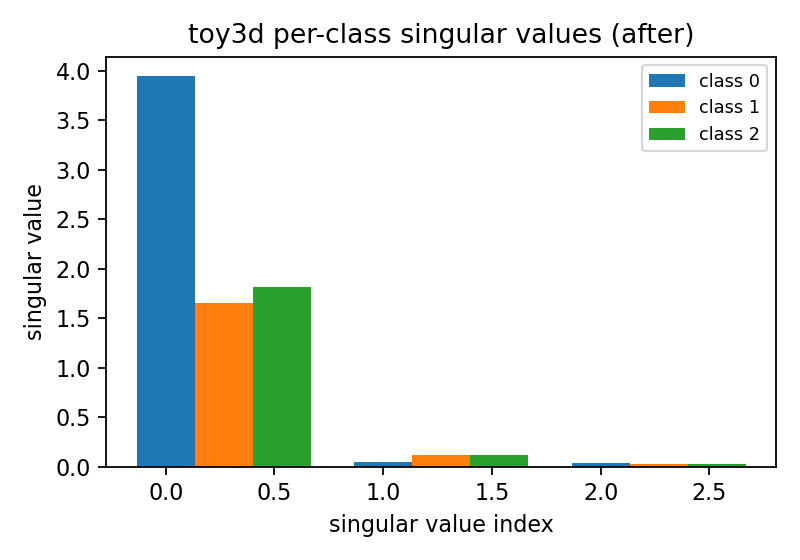
\includegraphics[width=\linewidth]{part1_toy/toy3d_singvals.png}\caption{Per-class $\sigma_i$}
\end{subfigure}
\caption{3D toy: three classes lying on non-orthogonal lines. OLT
reduces inter-class direction overlap from $|\cos|\!\in\![0.46,0.70]$
to $|\cos|\!\in\![0.01,0.14]$ and forces each class to a single
dominant direction (rank-$1$ singular spectrum).}
\label{fig:toy3d}
\end{figure}

\begin{figure}[h]
\centering
\begin{subfigure}[t]{0.30\linewidth}
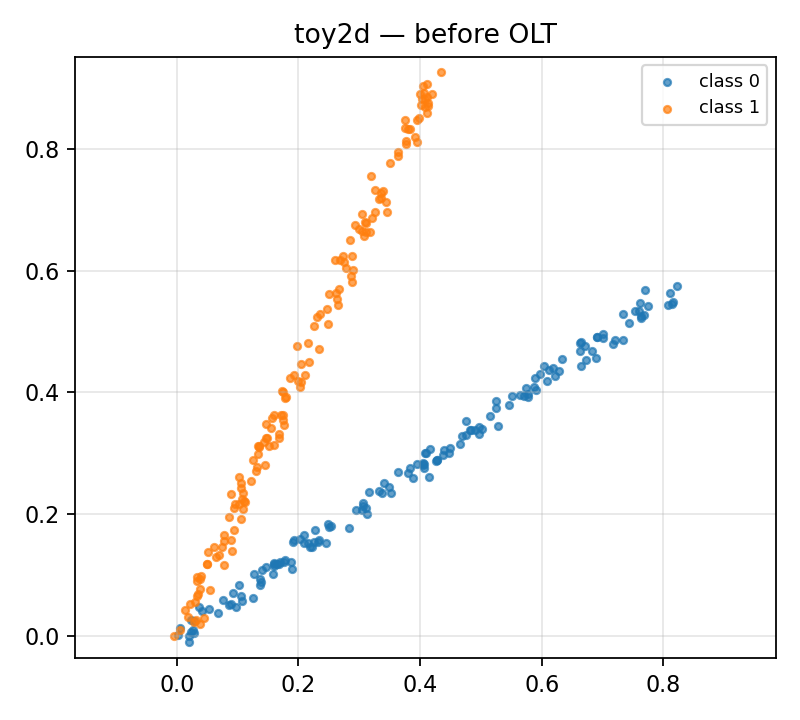
\includegraphics[width=\linewidth]{part1_toy/toy2d_before.png}
\end{subfigure}
\begin{subfigure}[t]{0.30\linewidth}
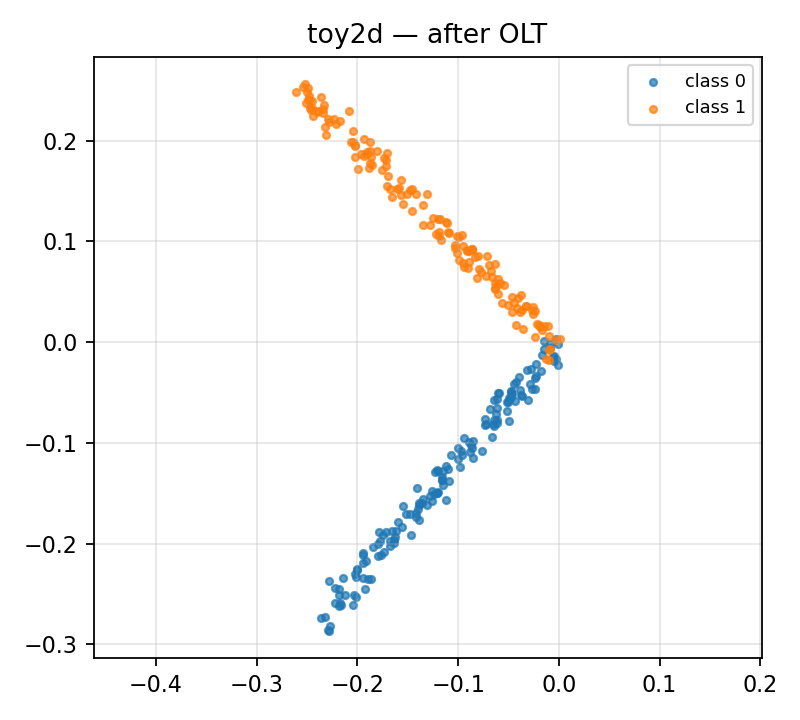
\includegraphics[width=\linewidth]{part1_toy/toy2d_after.png}
\end{subfigure}
\begin{subfigure}[t]{0.30\linewidth}
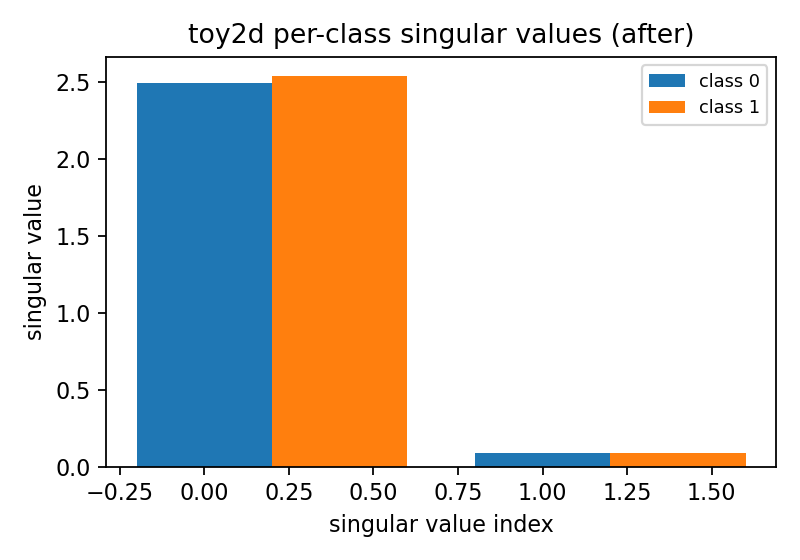
\includegraphics[width=\linewidth]{part1_toy/toy2d_singvals.png}
\end{subfigure}
\caption{2D toy. Inter-class $|\cos|$ falls from $0.86$ to $0.08$.}
\label{fig:toy2d}
\end{figure}

\subsection{Task 2 -- YaleB classification, OLT vs.\ LDA}

\paragraph{Setup.} Extended YaleB (38 subjects, 64 illumination
conditions each, $48\times 42$ pixels) is fetched by
\texttt{scripts/download\_yaleb.py}. We use a stratified $50/50$
train/test split, project onto the top $150$ PCA components fit on the
training set ($98.8\%$ explained variance), and rescale features so the
mean row norm is $\approx 1$. The OLT solver targets $d_{\text{out}}=64$
with $60$ outer CCCP iterations and $8$ inner subgradient steps at
step size $0.5$.

\paragraph{Classification rule.} For every class $c$ we form an
orthonormal basis $B_c$ of the transformed training features (singular
energy~$\ge 0.95$), and assign each test sample $x$ to
$\hat{c}=\argmin_c \|(I-B_cB_c^{\top})\,\T x\|_2$ -- the
\emph{nearest-subspace classifier}. This rule is the natural inference
counterpart of the nuclear-norm-low-rank objective: it picks the class
whose linear subspace explains the test sample best.

\begin{table}[h]
\centering
\begin{tabular}{lc}
\toprule
Method                                  & Test accuracy \\
\midrule
PCA + nearest centroid                  & $0.1201$ \\
PCA + nearest subspace                  & $0.8429$ \\
LDA                                     & $0.9095$ \\
\textbf{OLT + nearest subspace (ours)}  & $\mathbf{0.9490}$ \\
OLT + nearest centroid                  & $0.7492$ \\
\bottomrule
\end{tabular}
\caption{YaleB classification accuracy. OLT followed by the nearest
subspace rule outperforms LDA by $\sim 4$ points.}
\label{tab:yaleb_cls}
\end{table}

\begin{figure}[h]\centering
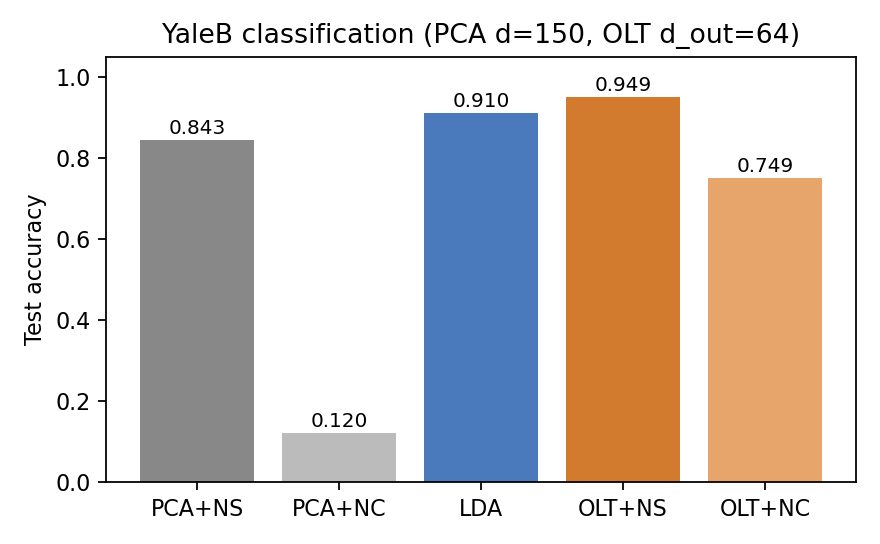
\includegraphics[width=0.55\linewidth]{part1_yaleb/yaleb_accuracy.png}
\caption{YaleB test accuracy by method.}
\label{fig:yaleb_acc}
\end{figure}

\subsection{Task 3 -- Subspace clustering on YaleB}

We follow the project's prescription \emph{``convert clustering into
classification via OLT''}:
\begin{enumerate}
\item Build a symmetric $k=7$ nearest-neighbour graph on the PCA
features and run spectral clustering with $C=38$ components to obtain
pseudo-labels.
\item Train OLT (same hyper-parameters as Task 2) using the
pseudo-labels as supervisory targets.
\item Apply the nearest-subspace classifier in the OLT-transformed
space to reassign every sample. The reassigned labels are the OLT
clustering output.
\end{enumerate}

\begin{table}[h]\centering
\begin{tabular}{lccc}
\toprule
Method & Acc (Hungarian) & NMI & ARI \\
\midrule
$k$-NN graph + spectral & $0.229$ & $0.279$ & $0.055$ \\
\textbf{OLT + nearest subspace} & $\mathbf{0.350}$ & $\mathbf{0.435}$ & $\mathbf{0.186}$ \\
\bottomrule
\end{tabular}
\caption{YaleB clustering with 38 ground-truth subjects. OLT refines
the noisy pseudo-labels into a substantially better partition.}
\label{tab:yaleb_clust}
\end{table}

\begin{figure}[h]\centering
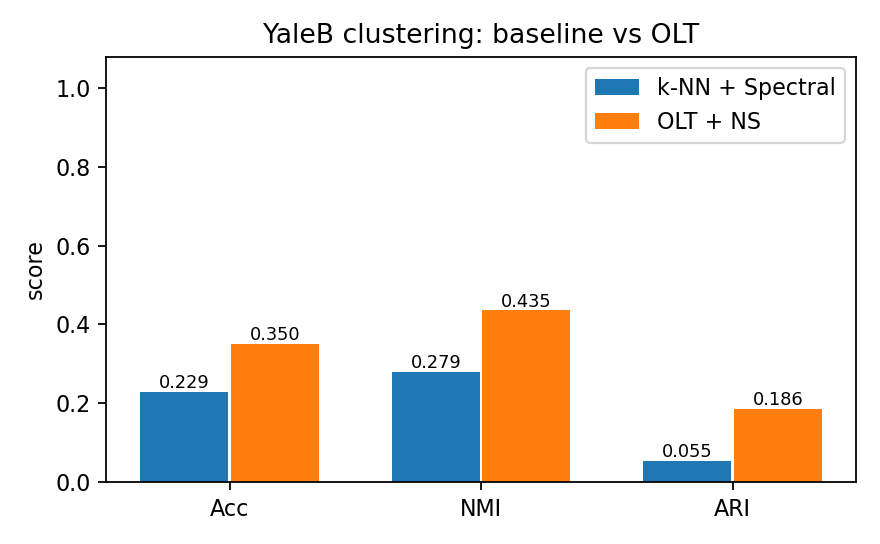
\includegraphics[width=0.55\linewidth]{part1_yaleb/yaleb_clustering.png}
\caption{Clustering metrics.}
\end{figure}

\section{Part 2: Modality-Invariant OLT}

We use Original MNIST as modality~$o$ and Rotated MNIST (per-sample
random rotation in $[-45^\circ,+45^\circ]$) as modality~$r$. Inputs are
flattened, projected to the top $50$ PCA components fit on the original
training set, and rescaled. The OLT solver outputs $d_{\text{out}}=20$
with the same CCCP schedule as before.

\subsection{Task 1 -- Per-modality transforms}

We learn $\T_o$ on the original features and $\T_r$ on the rotated
features independently and evaluate each transform on both modalities
with the nearest-subspace classifier (results in
Table~\ref{tab:part2}, top two rows).

\subsection{Task 2 -- Joint transformation (feature concatenation)}
\label{sec:joint}

To enforce that both modalities live in the \emph{same} per-class
subspace, we concatenate the two modalities along the sample axis as
$\Y_c^{\text{joint}}=[\Y_c^{o},\Y_c^{r}]$ and apply the standard OLT
problem~\eqref{eq:olt}:
\begin{equation}
\min_{\T}\;\sum_{c=1}^{C}\nuc{\T \Y_c^{\text{joint}}}\;-\;\nuc{\T\Y^{\text{joint}}}.
\label{eq:joint}
\end{equation}
By \eqref{eq:perp} the minimum drives the joint per-class block to a
single low-rank subspace shared by both modalities, which is exactly
the modality-invariance property we want.

\begin{table}[h]\centering
\begin{tabular}{lcc}
\toprule
Transform & Test acc.\ on orig & Test acc.\ on rot \\
\midrule
$\T_o$ (per-modality) & $0.6975$ & $0.4745$ \\
$\T_r$ (per-modality) & $0.5585$ & $0.5155$ \\
$\T_{\text{joint}}$ (\S\ref{sec:joint}) & $\mathbf{0.7450}$ & $\mathbf{0.6355}$ \\
\bottomrule
\end{tabular}
\caption{MNIST cross-modality test accuracy. The joint transform is
the best on \emph{both} modalities, and improves the cross-modality
case ($\T_o\to\!$rot) by $+16$ points.}
\label{tab:part2}
\end{table}

\begin{figure}[h]\centering
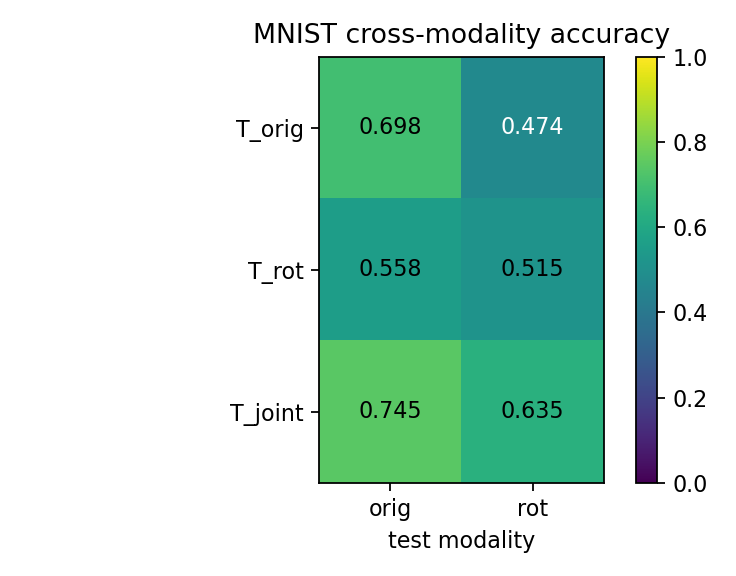
\includegraphics[width=0.40\linewidth]{part2/mnist_cross_modality.png}
\caption{MNIST cross-modality accuracy heatmap. Rows are transforms,
columns are test modalities.}
\end{figure}

\subsection{Task 3 -- Joint OLT on frozen CNN features}

We train the standard \texttt{pytorch/examples} MNIST CNN
(\texttt{conv32}-\texttt{conv64}-\texttt{fc128}-\texttt{fc10}) for 10
epochs with Adadelta on the original MNIST training set
(\texttt{scripts/train\_part2\_cnn.py}, run on a GPU server). The
network is then frozen and the $128$-d penultimate features are
extracted for both modalities. We learn a joint OLT on the
concatenated features and re-classify the test sets with
nearest-subspace.

\begin{table}[h]\centering
\begin{tabular}{lcc}
\toprule
Method & Original MNIST & Rotated MNIST \\
\midrule
Frozen CNN (baseline)            & $0.9924$ & $0.8639$ \\
Frozen CNN $+$ joint OLT $+$ NS  & $0.9850$ & $\mathbf{0.8811}$ \\
\bottomrule
\end{tabular}
\caption{The joint OLT applied on top of the frozen CNN trades a small
$-0.7$ on the in-distribution test set for a $+1.7$ on the
unseen rotated test set, confirming that the modality-invariant
construction transfers to learned features.}
\end{table}

\begin{figure}[h]\centering
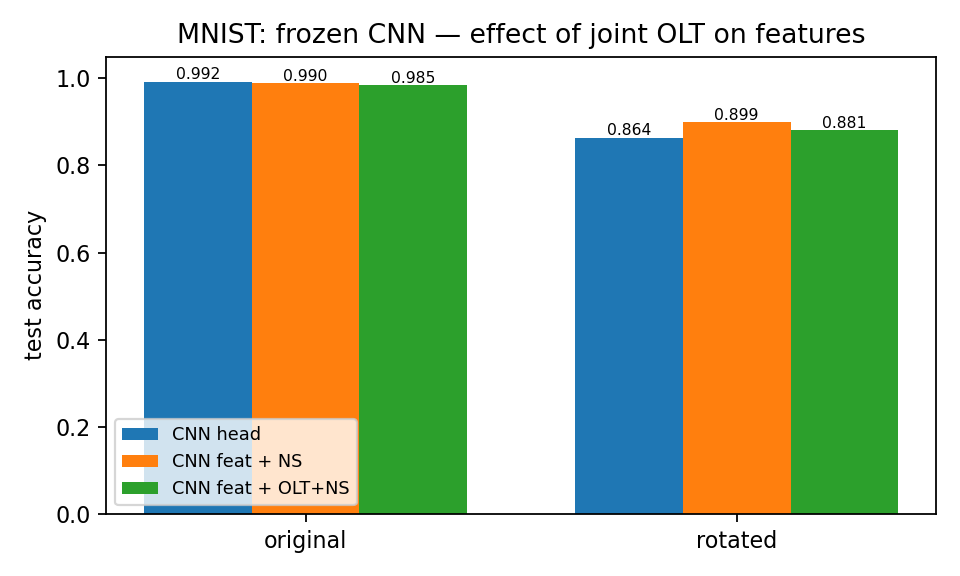
\includegraphics[width=0.45\linewidth]{part2/mnist_frozen_vs_olt.png}
\end{figure}

\section{Part 3 (Option A): OLT as a neural-network regularizer}

\subsection{Motivation}

Sections~3 and~4 establish OLT as a powerful linear post-hoc
embedding. A natural follow-up is to bake the same geometric prior
into the feature extractor itself: rather than retro-fit
low-rank/orthogonal structure with $\T$ after training, we ask the
network to learn features that are already low-rank intra-class and
orthogonal between classes.

\subsection{Loss function}

Let $f_\theta(x)\in\mathbb{R}^d$ be the penultimate feature of a CNN
classifier with linear head $W$. For a mini-batch $\mathcal{B}$ of
$|\mathcal{B}|$ samples with feature matrix $\F_{\mathcal{B}}\in
\mathbb{R}^{|\mathcal{B}|\times d}$ and labels $y_{\mathcal{B}}$, define
\begin{equation}
\mathcal{L}_{\text{OLT}}(\F_{\mathcal{B}},y_{\mathcal{B}})
\;=\;\frac{1}{|\mathcal{B}|}\!\left(\sum_{c=1}^{C}\nuc{\F_{\mathcal{B},c}}-\nuc{\F_{\mathcal{B}}}\right),
\label{eq:olt_nn}
\end{equation}
the same nuclear-norm OLT functional as in \eqref{eq:olt}, applied
directly to the network's mini-batch features. The total training loss
is
\begin{equation}
\mathcal{L}\;=\;\underbrace{\mathrm{CE}(W f_\theta(x),y)}_{\text{cross-entropy}}
\;+\;\lambda\,\mathcal{L}_{\text{OLT}}(\F_{\mathcal{B}},y_{\mathcal{B}}),
\quad\lambda\ge 0.
\end{equation}
Because PyTorch's \texttt{torch.linalg.svd} is differentiable, the
gradient of $\mathcal{L}_{\text{OLT}}$ flows all the way back to
$\theta$. Implementation: \texttt{olt/losses.py}, \texttt{OLTLoss}.

\paragraph{Justification.}
\begin{itemize}
\item The first term in \eqref{eq:olt_nn} compresses each class to a
low-rank manifold, encouraging tighter, more discriminative
clusters.
\item Subtracting the global $\nuc{\F_{\mathcal{B}}}$ exploits
property~\eqref{eq:perp}: minimisation pushes the non-negative gap
toward zero, i.e.\ toward orthogonal class subspaces. Orthogonality
acts as a strong margin in the latent space, complementary to the
softmax decision boundary.
\item In contrast to additive margin losses (e.g.\ ArcFace), the OLT
regularizer is fully \emph{geometric}: it constrains the entire
class subspace, not only its mean direction. This makes it more
robust to within-class variation -- precisely the situation
modelled by rotation.
\end{itemize}

\subsection{Experimental setup}

Same CNN architecture as Part~2 Task~3. Identical seeds, batch size,
optimizer (Adadelta, $\eta=1.0$, $\gamma=0.7$), and 10 training epochs
on Original MNIST. We sweep
$\lambda\in\{0.0,\,0.1,\,0.5,\,1.0\}$ and evaluate every variant on
the clean and rotated test sets, plus a feature-orthogonality
diagnostic
\[
r\;=\;\frac{\nuc{\F}}{\sum_c\nuc{\F_c}}\;\in\;[0,1],
\]
which equals $1$ exactly when the class feature subspaces are mutually
orthogonal.

\subsection{Results}

\begin{table}[h]\centering
\begin{tabular}{ccccc}
\toprule
$\lambda$ & Orig acc & Rot acc & $r$ (orthogonality) & Notes \\
\midrule
$0.0$ & $0.9919$ & $0.8582$ & $0.577$ & baseline (pure CE) \\
$0.1$ & $\mathbf{0.9921}$ & $\mathbf{0.8653}$ & $0.812$ & \textbf{best trade-off} \\
$0.5$ & $0.9914$ & $0.8598$ & $0.947$ & saturated geometry \\
$1.0$ & $0.7926$ & $0.6195$ & $0.971$ & CE dominated; collapse \\
\bottomrule
\end{tabular}
\caption{Effect of the OLT regularizer on the MNIST CNN.}
\label{tab:part3}
\end{table}

\begin{figure}[h]\centering
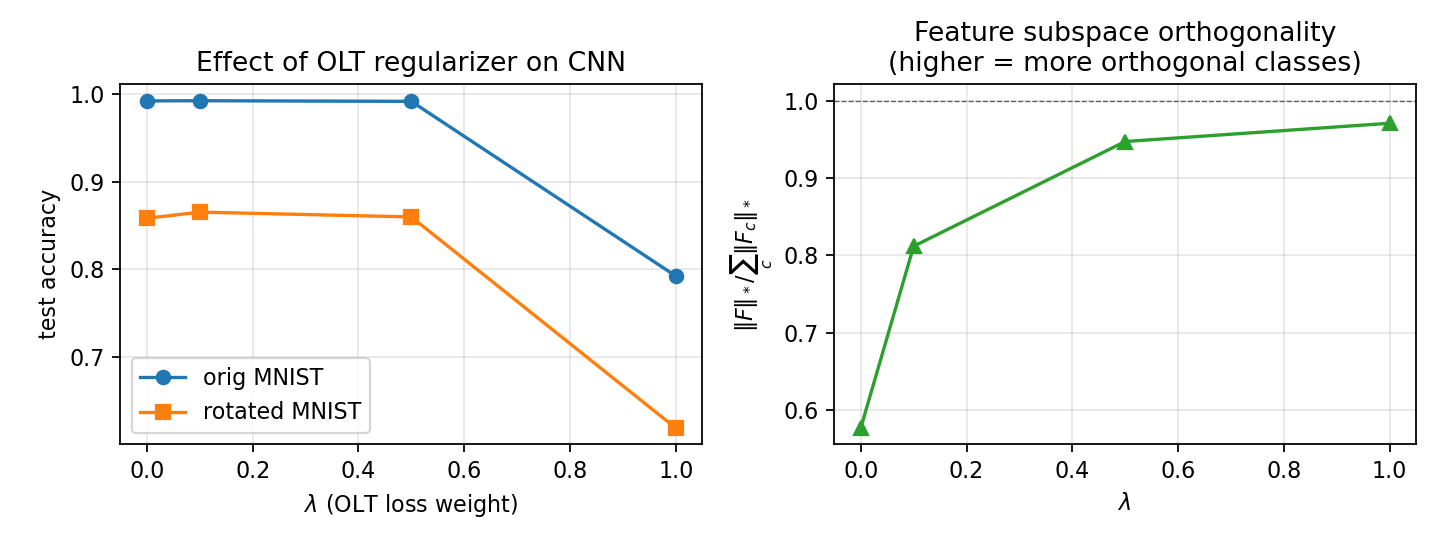
\includegraphics[width=0.95\linewidth]{part3/part3_lambda_sweep.png}
\caption{Left: clean and rotated MNIST accuracies as a function of
$\lambda$. Right: the orthogonality measure $r$ saturates toward $1$
as $\lambda$ grows, confirming the regularizer reshapes the feature
geometry as designed.}
\end{figure}

\subsection{Discussion}

A small $\lambda=0.1$ matches baseline accuracy on the in-distribution
test set ($+0.02$ pt) and improves the unseen rotated MNIST by
$+0.71$ pt while raising $r$ from $0.58$ to $0.81$. Larger $\lambda$
continues to push the geometry toward perfect orthogonality
($r\!\approx\!0.97$ at $\lambda=0.5$) but with no further accuracy
gain, and at $\lambda=1.0$ the OLT term overwhelms the cross-entropy
signal and training collapses. The picture is consistent with the
intended interpretation of the regularizer: it shapes \emph{how} the
features cluster but does not by itself supervise their semantic
labels. A modest $\lambda$ that nudges the geometry without dominating
the data fitting term gives the best of both worlds.

\paragraph{Limitations.} The regularizer requires several SVDs per
mini-batch ($C+1$ of them), so per-step cost is roughly
$1.5\!\times$ vanilla CE. The method also assumes that each
mini-batch contains enough samples per class to estimate
$\nuc{\F_c}$ stably -- relevant when $C$ grows large.

\section{Conclusion}

OLT couples intra-class rank suppression with inter-class
orthogonality through a single nuclear-norm objective and admits a
clean CCCP solver. Across very different settings -- toy data, face
classification, face clustering, multi-modal MNIST, frozen CNN
features, and end-to-end CNN training -- the same prior delivers
consistent gains: it beats LDA on YaleB, more than doubles ARI in 38-way
unsupervised face clustering, lifts cross-modality MNIST accuracy
by 16 points, and improves rotation-perturbed test accuracy of a CNN
when used as a soft regularizer.

\section*{Code and reproducibility}

All experiments are reproduced by the scripts in
\texttt{scripts/} of the project repository. Heavy training was
performed on a GPU server using the workflow in
\texttt{scripts/train\_part2\_cnn.py} and
\texttt{scripts/train\_part3\_olt\_nn.py}; everything else runs on
CPU within minutes.

\end{document}
